\section{Design and development of the Body}
The development of a device usually involves several steps, starting with the design phase. In this phase, a decision must first be made as to how the device should look in view of the requirements that are set. The requirement to have 21 chambers is of particular interest in this context, as it significantly restricts the design options. However, this restriction should be viewed positively, as the requirements for the first steps seem to be too low. There are no requirements regarding the physical characteristics of the device, such as size or weight. This opens up a remarkably wide scope for design with regard to the external appearance of the device.

Based only on the information we have at hand, there are already some initial ideas about what the device might look like, each with its own advantages and disadvantages. Here is a brief overview of the possible designs we have come up with.

\subsection{Early Ideas}
\subsubsection{Pill Dispense System}
When thinking about how the pills should be dispensed, a number of ideas inspired by the environment emerged. Below you will find brief descriptions of the systems and also an image \ref{fig:designs} of what they would look like. Please note that we are not going into too much detail here as they were the result of a brainstorming session and after all that, only one idea would be developed moving forward, albeit with certain inspirations from ideas that were dismissed.
\begin{itemize}
	\item The \textbf{Revolver} system was the simplest, and it didn't take long to come up with this idea, because such devices had already been developed\cite{LiveFinePillDispenser}. Its advantages are the simplicity of the mechanism, the robustness and the low price, while a disadvantage is its size and it requires a motor to drive a fairly large wheel.
	\item The second design is that of the \textbf{Carousel}. The main idea is that it is much smaller and uses space more efficiently than the revolver system. The smaller wheels would rotate at a lower speed than the main arm that holds them, as they are attached to the main axle with a reduction gear and a belt. Although it is slightly more space efficient than a revolver system, it is much more complex and still requires a motor to control the entire structure.
	\item The third design is that of the \textbf{conveyor belt}. On the image \ref{fig:designs} you can see that it is round, but it could theoretically also be designed elliptically or with other, more complex curves. The principle is as follows: An output chamber is attached to the belt, which moves a series of these chambers along a specific path. It is similar to the revolver system, but the chambers would be removable and the conveyor belt would allow some flexibility in the design of the device. The main disadvantages are the need for a motor, the need for a chamber management system and the overall complexity of the device.
	\item The fourth design is inspired by \textbf{vending machines}. It would have 21 chambers, each with an electromagnet attached. Each time a pill is to be dispensed, the electromagnet is activated, causing the chamber to move and the pills to fall onto the dispensing area. In this design, the stepper motor becomes redundant, but simplicity is lost as a logical circuit is required to connect 21 chambers in parallel. Theoretically, a parallel circuit would be advantageous, but this is not the case for us, as we cannot leverage this advantage sensibly.
\end{itemize}
\subsubsection{Pill Disposal System}
The idea for the Disposal system at the time was that it would mirror the dispensing system, either by being positioned directly underneath it or in such a way that the tablets would first fall onto a ramp, which after a certain time would be transported into the return mechanism by another action. It is not difficult to see that the choice of disposal system is highly dependent on the dispensing system we develop, so a more detailed description will be given later when we look in more detail at the chosen dispense system.
\begin{figure}[h]
	\centering
	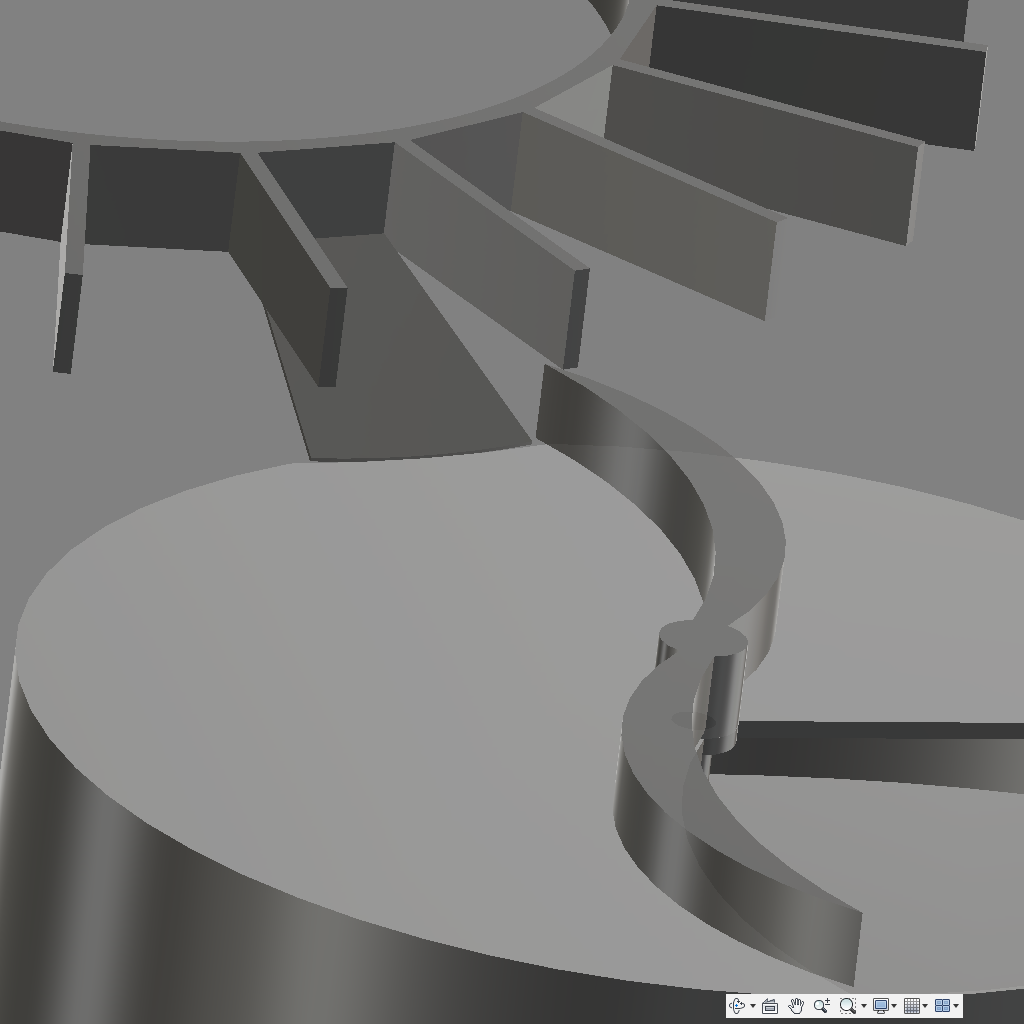
\includegraphics[width=0.7\linewidth]{Figures/Screenshot_1.png} 
	\caption[Early drafts]{Initial ideas on how the main structure (dispenser) of the device should look. 1. Revolver system. 2. carousel system. 3. conveyor system (running sushi). 4 Vending machine system}
	\label{fig:designs}
\end{figure}
\newpage
\subsection{Selection of the Design}
Of all the proposed designs, the revolver system seemed to be the most sensible choice, but it required some improvements in the design. A brief market research (e.g. \cite{LiveFinePillDispenser} \cite{zoksi_pill_organizer}) showed that there is not really such a system that would meet the above requirements of having a built-in disposal mechanism. For this reason, the design would have to be improved.
\subsubsection{Improvements to the turret system}
Now that we have chosen the main mechanism, we need to work out the details. The design philosophy was to make it as simple as possible, with as few moving details as possible. The first ideas were not very successful in this respect. In the picture \ref{fig:screenshot1} you can see what the earlier ideas would look like. In such a design, each chamber would have its own door, under that door would be a notch for the lever to fall into to open it. The pills would then fall into the disposal tray. After a certain amount of time (15 minutes), the S-shaped arm would rotate and drop the pills further down the ramp into the disposal storage. This solution had numerous disadvantages:
\begin{enumerate}
	\item{\textbf{Too many moving parts}}
	
	Each chamber has 21 doors. The doors need a lever to open (22), this lever needs to be translationally engaged and disengaged in the notch (23), the revolver mechanism needs to rotate (24), the disposal arm also needs to rotate (25, but the idea was to synchronize it with the main axis using belts), the disposal chambers would also need to rotate (26). Although this was a solution, it was not optimal given the number of moving parts. Although the dispensing chambers, the disposal chambers and the disposal arm would rotate around the same axis, the rotation and translation of the lever for an opening would require a complex mechanism that would further increase the effort.
	\item{\textbf{Requires a large dispenser bowl}}
	
	The disposal mechanism itself is already quite large (a diameter of 300 mm was measured for this prototype). If another horizontal surface were added next to this surface, even if it were only half the size (a reduction in size would make it difficult for people with motor disorders to remove the pills safely), the entire system would become extremely large.
	\item{\textbf{Contains several small objects}}
	
	This is not an obvious disadvantage, but each trapdoor must rotate around a specific axis. This axis must consist of either a small metal rod inserted into the openings of the door or 3D printed teeth on the design of the door itself. The first solution requires a daring and precise assembly of 21 doors, the second requires a high level of 3D printing precision that cannot be achieved by conventional means.
\end{enumerate}
Due to these disadvantages, the system was discarded and never further improved. However, one important lesson was learned: if we want to have the simplest design, we have to utilize the power of gravity.
\begin{figure}[h]
	\centering
	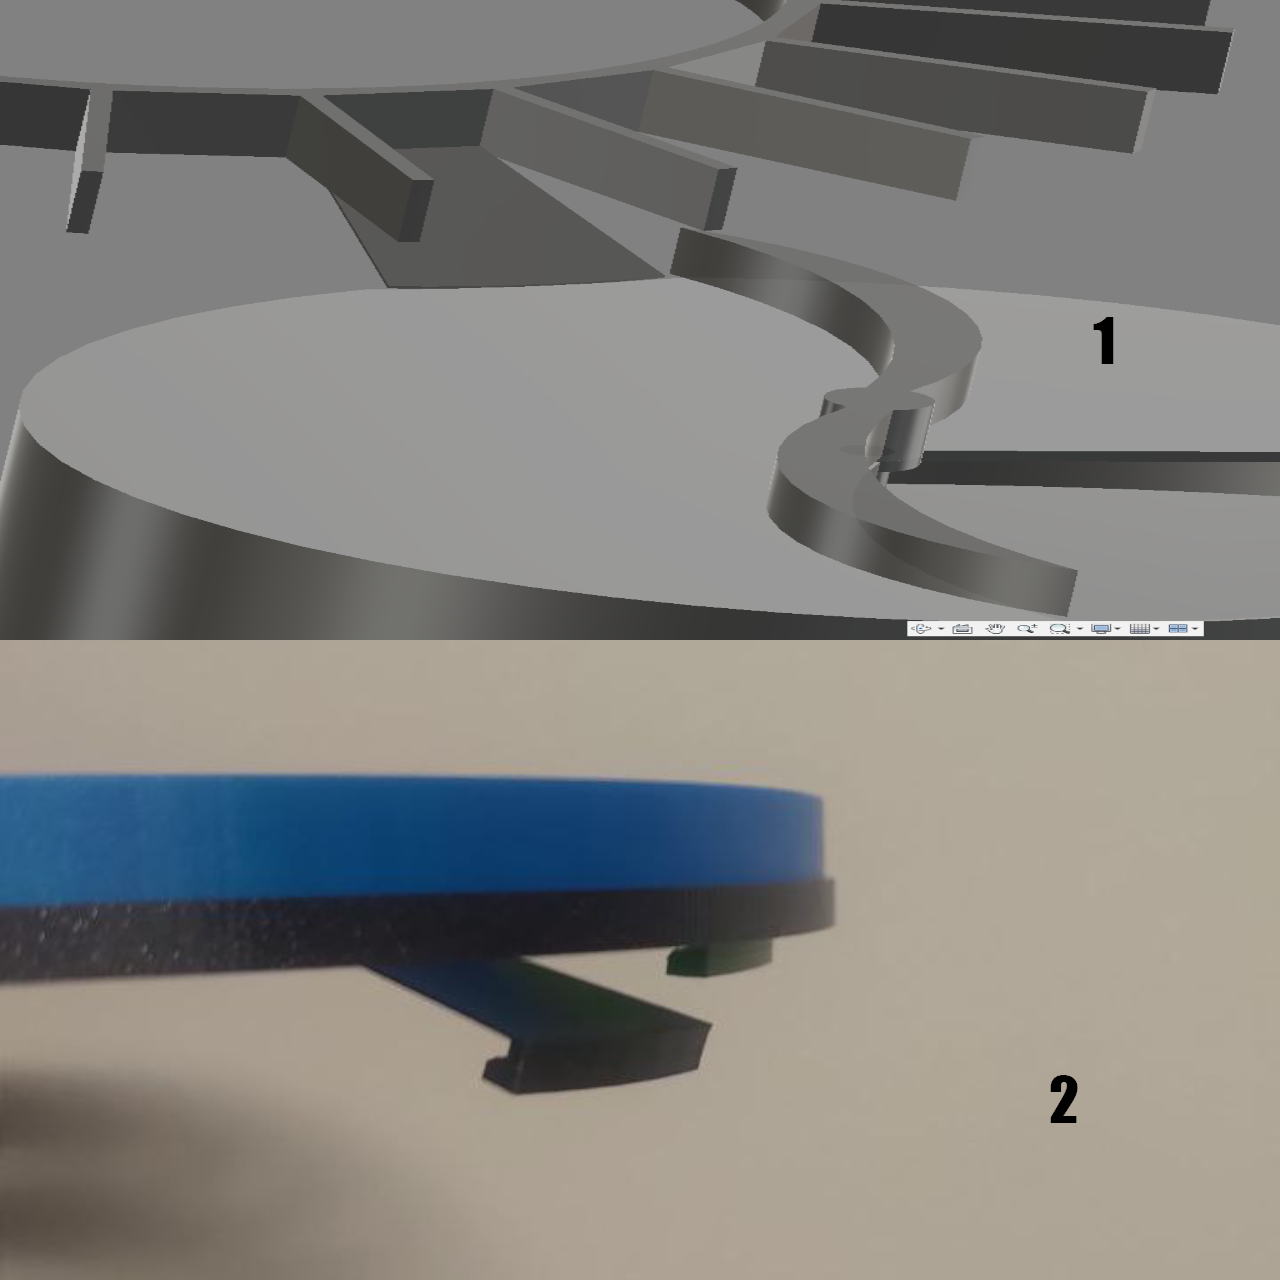
\includegraphics[width=0.7\linewidth]{Figures/Untitled-2}
	\caption[First revolver prototype]{First revolver prototype. Here you can see that initial idea was to have a trapdoor in each chamber which will release the pills onto the disposal dish by opening it.}
	\label{fig:screenshot1}
\end{figure}
\newpage
\subsubsection{Redesigning the Revolver System. A new approach}
Having realized that we need to get rid of the extra space that the separate body at the side of the main body takes, the new approach was required. This time, the disposal chambers would be directly underneath the dispensing chambers and we would use the power of gravity to move from one chamber to another, as you can see in the image \ref{fig:pspd2}. This would drastically reduce the amount of space the pill dispenser takes, significantly reduce complexity, setting all the rotating objects onto a single axis.


\begin{figure}[h]
	\centering
	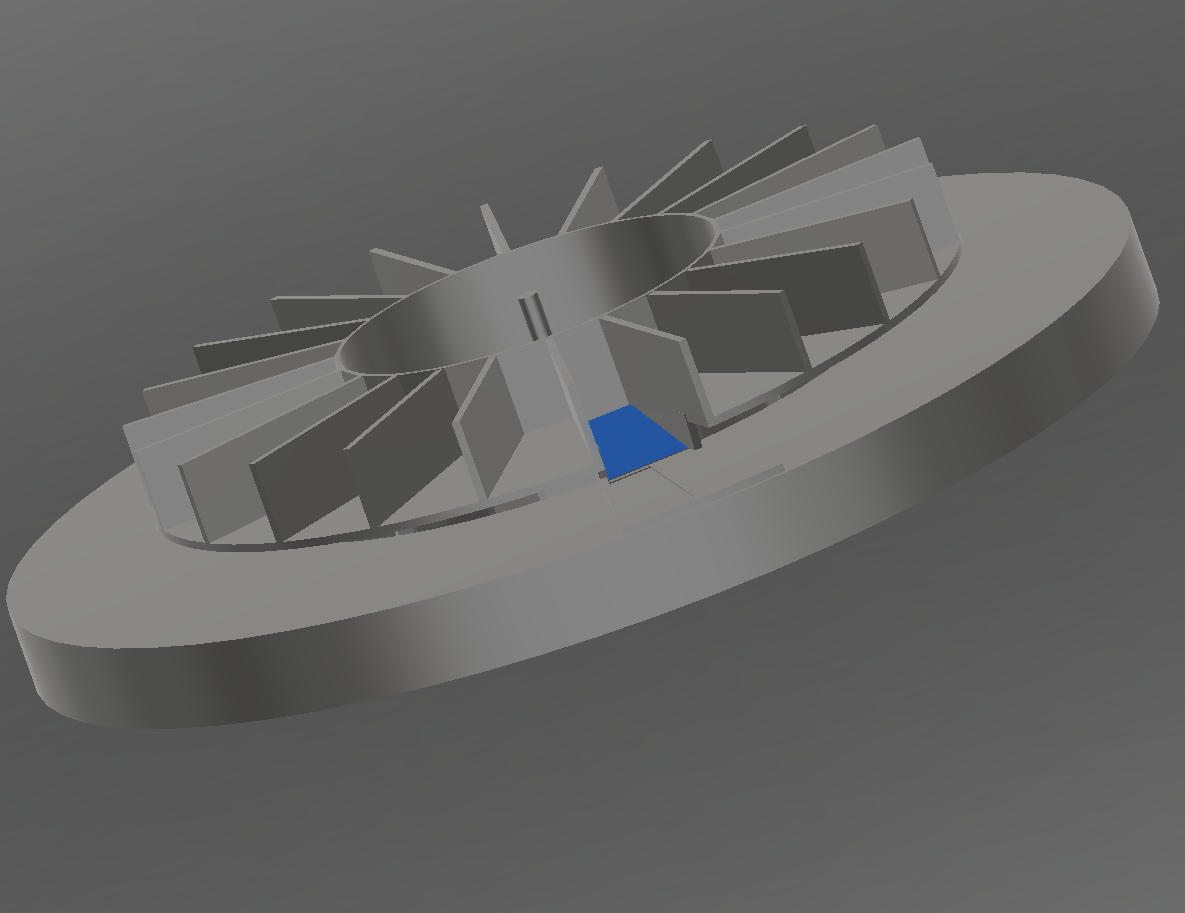
\includegraphics[width=0.7\linewidth]{Figures/PSPD2}
	\caption[2 Variant of the pill dispenser.]{Second variant of the pill dispenser.}
	\label{fig:pspd2}
\end{figure}

Because this system doesn't have a separate mechanism for removing unused pills, another new method would have to be developed for this too. In the image \ref{fig:screenshot2} you can see how the chambers of the disposal system look like. The cover of the disposal system has an opening (part 2 of the same image) that is shut when the pills have to be taken. When the upper mechanism rotates to dispose new pills, the lower mechanism rotates to send pills into disposal chamber simultaneously. Ridges are added to the cover of disposal system to prevent pills from accidentally rolling away.

\begin{figure}
	\centering
	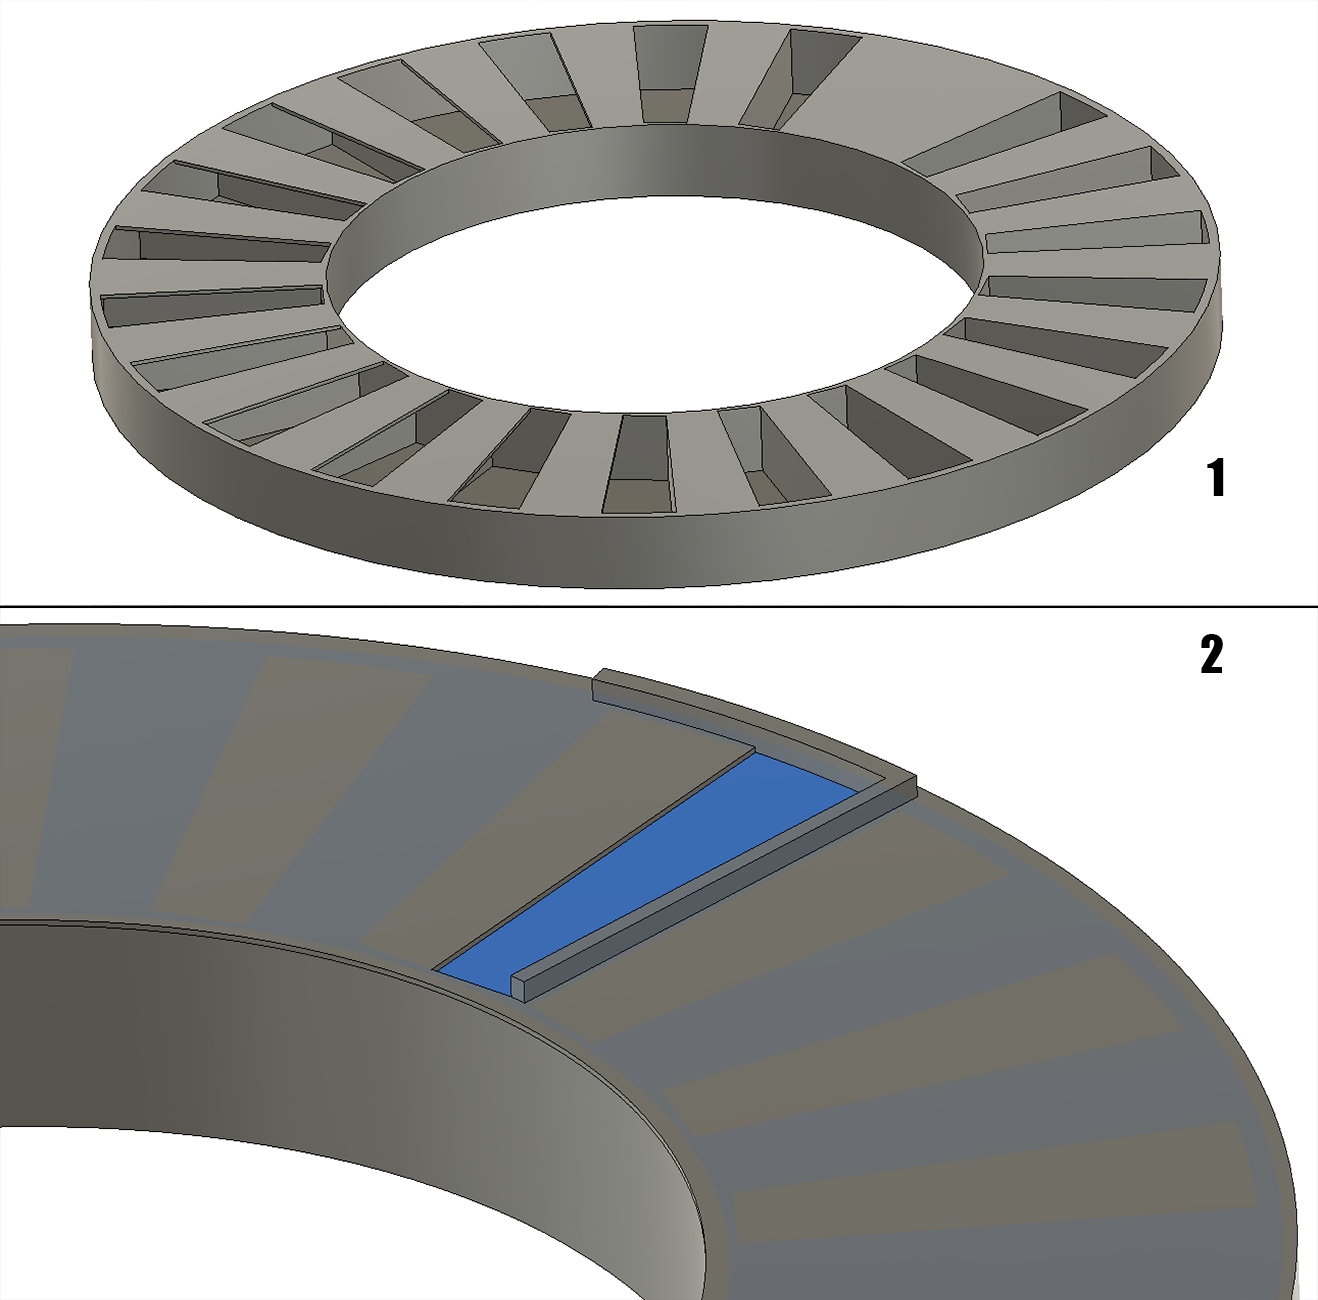
\includegraphics[width=0.7\linewidth]{Figures/PSPD2-Chambers}
	\caption[Disposal system of 2nd revolver system]{Disposal system of 2nd revolver system}
	\label{fig:screenshot2}
\end{figure}
\newpage
However, there are still ways to improve this approach. While much better than the previous one, this one also have some disadvantages:
\begin{enumerate}
\item \textbf{Chambers of the upper mechanism are smaller.} The chambers of pill storage are significantly smaller. We can calculate chamber volume using the following formulas:
\[
A = \pi r_1^2 - \pi r_0^2,\quad V = A \cdot h
\]
For the upper chamber: \( r_1 = 100\,\text{mm} \),\( r_0 = 47.5\,\text{mm} \), \( h = 18\,\text{mm} \), the result is:
\[
V = 437.90\,\text{cm}^3
\]
For the lower chamber:  \( r_1 = 135\,\text{mm} \), \( r_0 = 80\,\text{mm} \), \( h = 18\,\text{mm} \), the result is:
\[
V = 668.69\,\text{cm}^3
\]
As we can see, the lower chambers are almost 1.5 bigger than the upper ones, which is a waste that we might want to get rid of.
	\item{\textbf{Synchronous movement of both chambers}} This approach makes future development less flexible. independence of the chambers is a degree of freedom that we might want to keep somehow. The biggest problem with current approach is that it might lead to situations where some pills might fall too fast from the top to fall directly into an opening in time.
	\item{\textbf{Reliance on a ramp for pills to fall down.}} This can introduce an undesired behavior where some sticky pills might stick to the ramp and not fall down. This can lead to very dangerous scenario where a pill, not properly dispenced in time, would fall down with the next batch which would then lead to overdose.
\end{enumerate}

As mentioned earlier, this design is already what we would like to see as a final result, but we can improve it further, by redesigning it a bit and adressing the disadvantages we mentioned above.
\newpage

\subsubsection{The final Redesign. Improving on what's good.}
A few thoughts come to mind as a potential approach to the redesign. Using gravity is obviously good, we need to continue doing, however we might change how we use it. Having 2 systems one above another is also a great idea, what if we can make the chambers the same size? We could reposition the holes. Regarding synchronous movement, we have 2 types of direction of pill movement: From dispense to patient (intended behavior) and from dispense to disposal (backup behavior). The intended behavior implies human interaction, we can make some simple movement to deliver pills that would remove the need for synchronicity from our system. All these ideas are implemented in the final design, however it is worth mentioning that there has also been the intermediary step, where the dispense mechanism was rotated 90 degrees (see image \ref{fig:screenshot4}), so that it is completely vertical. It is worth giving a short overview of why this idea wasn't chosen as final:
\begin{itemize}
	\item{\textbf{Too tall}} the wheel with diameter of 100mm would be vertically positioned which takes a lot of space.
	\item{\textbf{Requires more torque}} A motor would have to directly resist the force of gravity to lift the pills up a mill
	\item{\textbf{Doesn't fix synchronicity}} The mechanisms are still locked together, this issue remains unresolved.
\end{itemize}
\begin{figure}[]
	\centering
	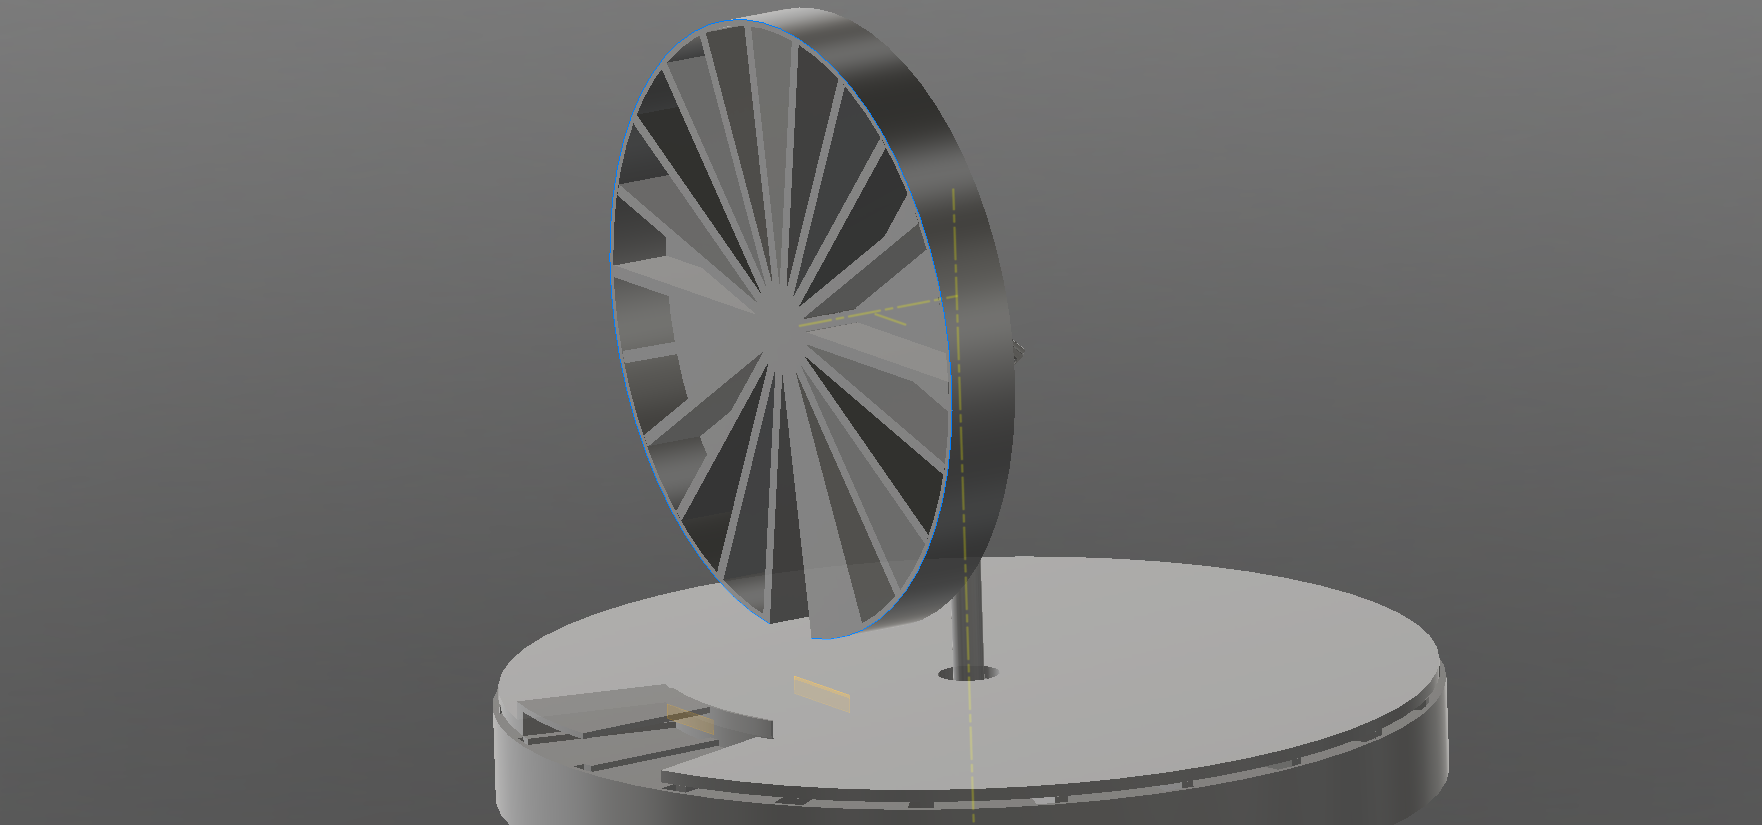
\includegraphics[width=0.6\linewidth]{Figures/Screenshot_4}
	\caption[Vertical Pill Dispenser.]{Pill dispenser with dispense system rotated vertically.}
	\label{fig:screenshot4}
\end{figure}
\newpage
For the final design, the following steps have been taken to address the issue:
\begin{enumerate}
	\item{\textbf{Resize the chambers}} Chambers size were changed so that they match. The result is device now has a cylindrical form where the chamber mechanisms are located directly on top of each other, maximising the space used
	\item{\textbf{Remove the ramp, change disposal mechanism}} The disposal mechanism was also changed. It works in tandem with dispense mechanism, which was also changed. The pills are now dispensed by the same movement by which they are made available, namely by rotation of the dispense mill. 
	\item{\textbf{Introduce a separate axis of rotation to dispense pills}} We will use tilting movement of the whole device for dispense of the pills into a cup or a hand of a patient, but for that we would have the whole construction elevated.
	\item{\textbf{Expand the device to include the stand}} As mentioned above, it needs to be elevated. The stand will provide not only the elevation, but also another axis of rotation, therefore decoupling the disposal and dispense mechanisms from one another.
\end{enumerate}
In the image \ref{fig:screenshot5} you can see the final design. It has all the features mentioned above already covered. In the next chapter we will go step by step into the details of the design and see how the proposed solutions were implemented.
\begin{figure}[]
	\centering
	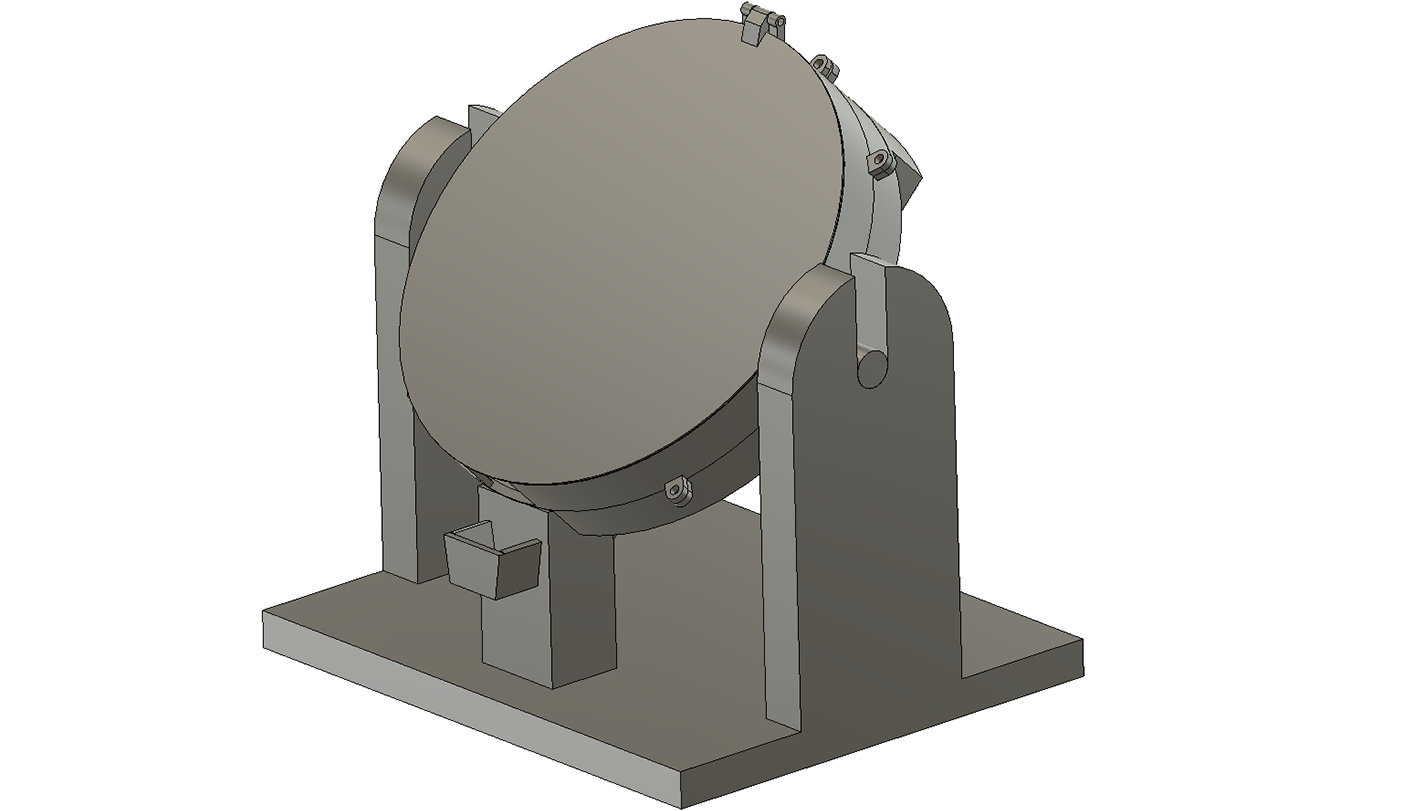
\includegraphics[width=0.6\linewidth]{Figures/Screenshot_5}
	\caption[Final result]{The final design of the Pill Dispenser.}
	\label{fig:screenshot5}
\end{figure}


